\section{Algoritmi golosi}

Si parla sempre di \textbf{problemi di ottimizzazione}.

\begin{figure}[htbp]
\centering
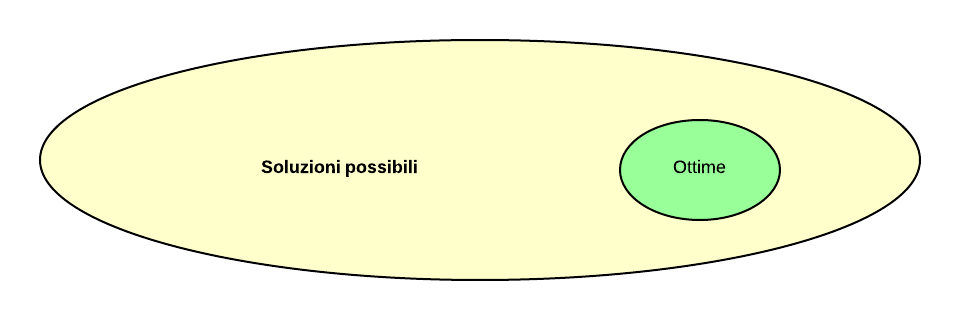
\includegraphics[width=100mm]{images/gready1.png}
\caption{Soluzioni di un problema}
\end{figure}

Se utilizziamo l'\textbf{enumerazione esaustiva}:

\begin{itemize}

\item Si generano tutte le soluzioni possibili;
\item Si calcola il costo di ciascuna di esse;
\item Se ne seleziona una di ottima.

\end{itemize}

Questo metodo è chiaramente efficace ma comporta \textbf{tempi esponenziali}, perchè l'insieme delle soluzioni è generalmente enorme.
\linebreak[2]
Un \textbf{algoritmo goloso} sceglie sempre una soluzione \textbf{localmente ottima}:

\begin{figure}[htpd]
\centering
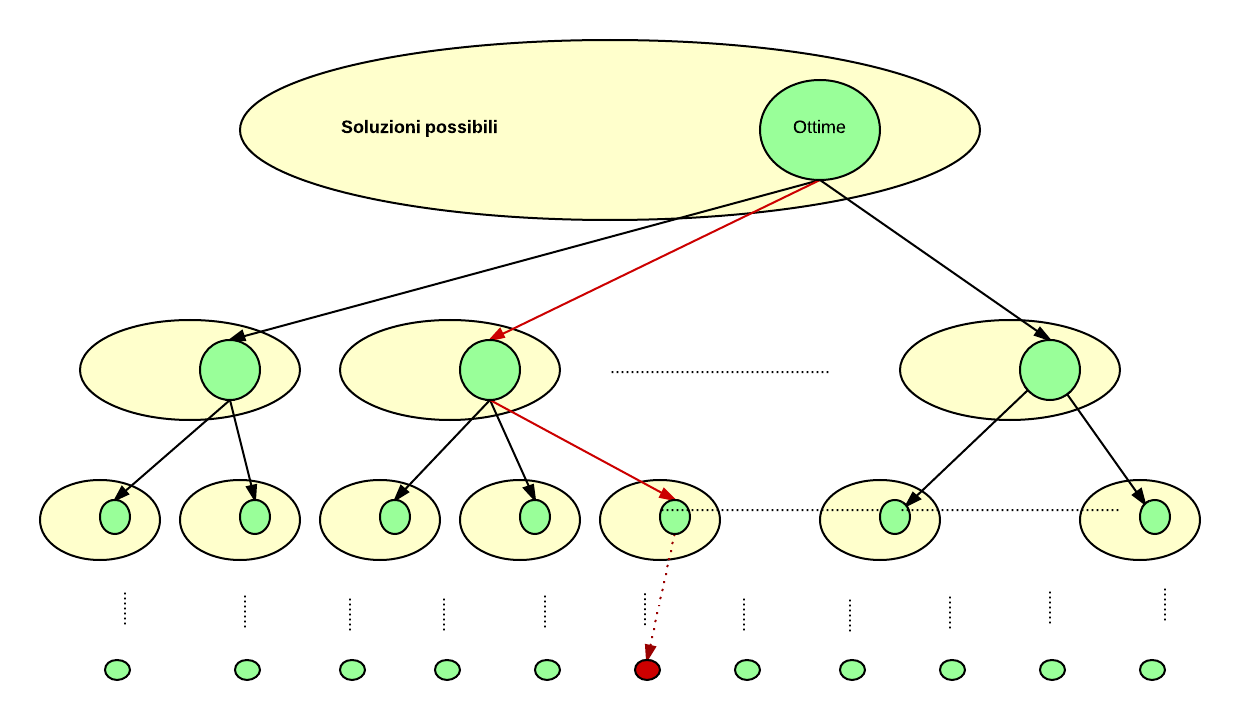
\includegraphics[width=130mm]{images/gready2.png}
\caption{Schema di un algoritmo goloso}
\end{figure}

\begin{enumerate}

\item Ogni volta si fa una scelta che sembra migliore localmente;
\item In questo modo per alcuni problemi si ottiene una soluzione globalmente ottima.

\end{enumerate}

\subsection{Problema della scelta di attività}

Un esempio tipico è quello del \textbf{problema della scelta di attività}. Supponiamo di avere a disposizione $n$ attività $a_1,a_2,...,a_n$ che utilizzano la stessa risorsa (ad esempio un'aula). Ciascuna attività ha un tempo di inizio $s_i$ e un tempo di fine $f_i$, con $0\le s_i < f_i < \infty$.

$a_i$ occupa la risorsa nell'intervallo $[s_i,f_i)$.

$a_i$ e $a_j$ sono \textbf{compatibili} se gli intervalli $[s_i,f_i)$ e $(s_j,f_j]$ sono disgiunti.
\linebreak[2]
Strategie golose:

\begin{itemize}

\item Scegliere l'attivitò che inizia per prima:

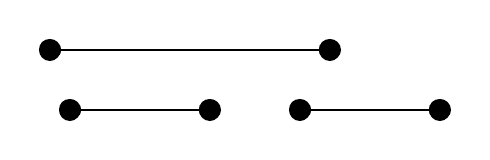
\includegraphics[width=50mm]{images/activity1.png}

Non funziona!

\item Scegliere l'attività che dura meno tempo:

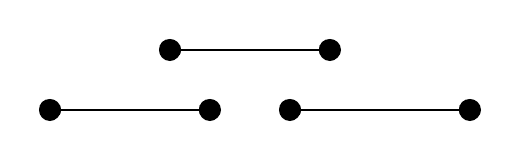
\includegraphics[width=50mm]{images/activity2.png}

Non funziona!

\item Scegliere l'attività incompatibile con il minor numero di altre attività:

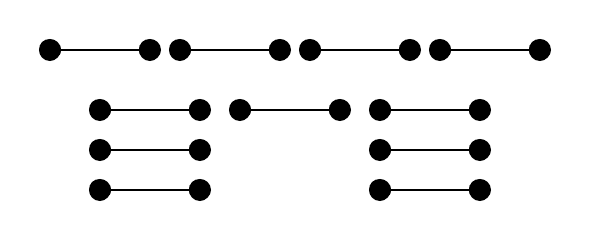
\includegraphics[width=50mm]{images/activity3.png}

Non funziona!

\end{itemize}

La strategia che funziona è quella di scegliere l'attività che \textbf{termina per prima}.

\begin{lstlisting}[mathescape=true,caption=Algoritmo di selezione delle attività]

ActivitySelector(a,s,f,n) // $f_1 \le f_2 \le ... \le f_n$
	A = {a1}, k=1
	for m=2 to n
		if s[m] >= f[k]
			A = A "unito" {am}, k = m
	return A

\end{lstlisting}

Sappiamo che durante tutta l'esecuzione dell'algoritmo esiste sempre una soluzione ottima contenente le attività scelte fino a quel momento. L'algoritmo è goloso, perchè ad ogni passo sceglie l'attività che termina prima. Questa scelta è \textbf{localmente ottima}, perchè è quella che lascia più tempo a disposizione per le attività successive.

\subsection{Problema dello zaino frazionario}

Dati $n$ tipi di merce, $M_1,M_2,...,M_n$ in quantità $q_1,q_2,...,q_n$ e con costi unitari $c_1,c_2,...,c_n$ si vuole riempire uno zaino di capacità $Q$ in modo che il contenuto abbia costo massimo.

\begin{lstlisting}[mathescape=true,caption=Algoritmo goloso dello zaino frazionario]

RiempiZaino(q, c, n, Q) // $c_1 \ge c_2 \ge c_3 \ge ... \ge c_n$
	Spazio = Q
	for i=1 to n
		if Spazio >= q[i]
			Z[i] = q[i], Spazio = Spazio - Z[i]
		else
			Z[i] = Spazio, Spazio = 0
	return Z

\end{lstlisting}

\subsection{Problema del pulmino con numero fissato di posti}

Un'azienda di una grande città ha diverse agenzie. Su richiesta sindacale l'azienda ha istituito un servizio sperimentale di trasporto per i dipendenti che utilizza un solo pulmino con 10 posti. Al mattino il pulmino effettua un percorso prefissato che passa per tutte le agenzie raccogliendo gli $n$ dipendenti che hanno fatto richiesta nei punti del percorso per loro più comodi per portarli alle rispettive agenzie. Per ogni dipendente è noto il punto di partenza $s[i]$ e il punto di arrivo $f[i]$. Essendo il servizio sperimentale non ci si aspetta che tutte le richieste possano essere soddisfatte.

Descrivere un algoritmo goloso che determina un'assegnazione dei posti del pulmino che permette di trasportare il massimo numero di dipendenti. Naturalmente lo stesso posto può essere utilizzato da più dipendenti, purchè il loro tragitti non si sovrappongano.
\linebreak[2]
\textbf{Soluzione}: Ordiniamo i dipendenti per i punti di arrivo, dal più vicino al più lontano. La scelta golosa consiste poi nell'assegnare a ogni dipendente il posto che si è liberato per ultimo, in modo da massimizzare il numero di dipendenti.

\begin{lstlisting}[mathescape=true,caption=Algoritmo goloso del pulmino]

Pulmino(s, f, n, m) // PRE: $f_1 \le f_2 \le ... \le f_n$
	for j=1 to m
		$t_j$ = 0
	$t_0$ = -1
	for i=1 to n
		h = 0
		for j=1 to m
			if $s_i \ge t_j$ and $t_j \ge t_h$ then h = j
			// $A_h$ è il posto che si libera per ultimo tra quelli in cui è possibile far sedere una persona.
			// Se h == 0 in nessuno degli m posti si puo' far sedere una persona
		J[i] = h
		if h $\neq$ 0 then $t_h=f_i$
	// POST: J[1...n] è una programmazione ottima del massimo numero di persone che si possono trasportare con m posti.
	// J[i] == j $\neq 0$ significa che la persona non puo' sedersi in nessuno degli m posti
	return J

\end{lstlisting}